\documentclass[aspectratio=43]{beamer}
\usepackage[english]{babel}
%\usepackage[fntef]{ctex} % invole CJKfntef
\usepackage{ctex}
\usepackage{fontspec}
\setmainfont{CMU Serif}

\usepackage{mathrsfs}
\usepackage{amssymb,amsmath, amsthm,bm}
\usepackage{mathtools}
\usepackage{amsthm}
\usepackage{mathtools}
\usepackage{bm}
\usepackage{physics}
\usepackage{calligra}
\usepackage{csquotes}
\usepackage{tensor}
\usepackage[thicklines]{cancel}
\usepackage{tcolorbox}
\usepackage{pstricks}
\usepackage[backend=biber, bibstyle=nature, sorting=nty, citestyle=numeric-comp]{biblatex} %Custom bibliography
    \addbibresource{bib.bib} %Load references


\DeclareMathAlphabet{\mathcalligra}{T1}{calligra}{m}{n}
\DeclareFontShape{T1}{calligra}{m}{n}{<->s*[2.2]callig15}{}
\newcommand{\scriptr}{\mathcalligra{r}\,}
\newcommand{\boldscriptr}{\pmb{\mathcalligra{r}}\,}
\def\rc{\scriptr}
\def\brc{\boldscriptr}
\def\hrc{\hat\brc}
\newcommand{\ie}{\emph{i.e.}} %id est
\newcommand{\eg}{\emph{e.g.}} %exempli gratia
\newcommand{\rtd}[1]{\ensuremath{\left\lfloor #1 \right\rfloor}}
\newcommand{\dirac}[1]{\ensuremath{\delta \left( #1 \right)}}
\newcommand{\diract}[1]{\ensuremath{\delta^3 \left( #1 \right)}}
\newcommand{\e}{\ensuremath{\epsilon_0}}
\newcommand{\m}{\ensuremath{\mu_0}}
\newcommand{\V}{\ensuremath{\mathcal{V}}}
\newcommand{\prnt}[1]{\ensuremath{\left(#1\right)}} %parentheses
\newcommand{\colch}[1]{\ensuremath{\left[#1\right]}} %square brackets
\newcommand{\chave}[1]{\ensuremath{\left\{#1\right\}}}  %curly brackets

\useoutertheme{infolines}
\useinnertheme{rectangles}
\usefonttheme{professionalfonts}


\definecolor{orange}{HTML}{1f4f94} %背景粉CC0099,蓝色1f4f94,绿色66CC33
\definecolor{gray}{HTML}{FFFFFF}	%底色白
\definecolor{yellow}{HTML}{6633FF}	%f0be52,红色FF0033 %\alert的颜色
\definecolor{lightorange}{HTML}{FF0033} %f19e58
\definecolor{textColor}{HTML}{000000} %黑

\renewcommand{\CancelColor}{\color{orange}}

\makeatletter
\newcommand{\mybox}[1]{%
  \setbox0=\hbox{#1}%
  \setlength{\@tempdima}{\dimexpr\wd0+13pt}%
  \begin{tcolorbox}[colback=orange,colframe=orange,boxrule=0.5pt,arc=4pt,
      left=6pt,right=6pt,top=6pt,bottom=6pt,boxsep=0pt,width=\@tempdima]
    \textcolor{white}{#1}
  \end{tcolorbox}
}
\makeatother

\usecolortheme[named=orange]{structure}
\usecolortheme{sidebartab}
\usecolortheme{orchid}
\usecolortheme{whale}
\setbeamercolor{alerted text}{fg=yellow}
\setbeamercolor{block title alerted}{bg=alerted text.fg!90!black}
\setbeamercolor{block title example}{bg=lightorange!60!black}
\setbeamercolor{background canvas}{bg=gray}
\setbeamercolor{normal text}{bg=gray,fg=textColor}

\setbeamertemplate{footline}
        {
      \leavevmode%
      \hbox{%
      \begin{beamercolorbox}[wd=.333333\paperwidth,ht=2.25ex,dp=1ex,center]{author in head/foot}%
        \usebeamerfont{author in head/foot}\insertshortauthor~~(\insertshortinstitute)
      \end{beamercolorbox}%
      \begin{beamercolorbox}[wd=.333333\paperwidth,ht=2.25ex,dp=1ex,center]{title in head/foot}%
        \usebeamerfont{title in head/foot}\insertshorttitle
      \end{beamercolorbox}%
      \begin{beamercolorbox}[wd=.333333\paperwidth,ht=2.25ex,dp=1ex,center]{date in head/foot}%
        \usebeamerfont{date in head/foot}\insertshortdate{}%\hspace*{2em}

    %#turning the next line into a comment, erases the frame numbers
        %\insertframenumber{} / \inserttotalframenumber\hspace*{2ex} 

      \end{beamercolorbox}}%
  
      \vskip0pt%
    }


\setbeamertemplate{blocks}[rectangle]
\setbeamercovered{dynamic}

\setbeamertemplate{section page}
{
	\begin{centering}
		\begin{beamercolorbox}[sep=27pt,center]{part title}
			\usebeamerfont{section title}\insertsection\par
			\usebeamerfont{subsection title}\insertsubsection\par
		\end{beamercolorbox}
	\end{centering}
}

%\setbeamertemplate{subsection page}
%{
%	\begin{centering}
%		\begin{beamercolorbox}[sep=12pt,center]{part title}
%			\usebeamerfont{subsection title}\insertsubsection\par
%		\end{beamercolorbox}
%	\end{centering}
%}

\newcommand{\hlight}[1]{\colorbox{violet!50}{#1}}
\newcommand{\hlighta}[1]{\colorbox{red!50}{#1}}
\title{Linear Algebra--第零章} %->->->->-> Check hyperref title <-<-<-<-<-
\subtitle{代数学的经典课题}
\author[YY]{杨勇}
\institute[BUPT]{
	Beijing Univ. of Posts and Telecom.%
} %You can change the Institution if you are from somewhere else
\date{\today}
%\logo{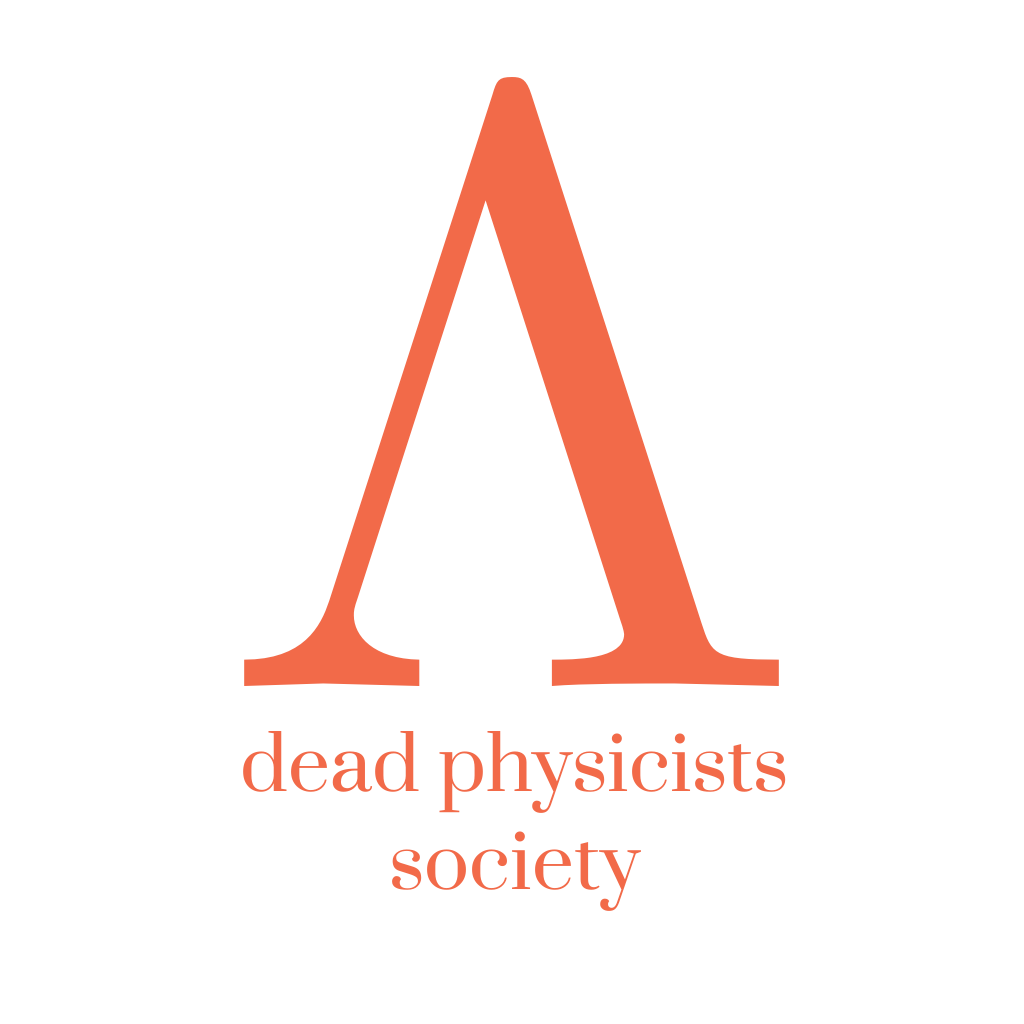
\includegraphics[width= 0.2\textwidth]{images/a-logo.png}}

\begin{document}
	
	\frame{\titlepage}
	
   \section{引言}
\begin{frame}{\textbf{引言}}
	代数学是一个历史悠久的数学分支, 它有着十分广泛的应用领域. 从本来的意义上说, 代数学研究数和它的加、减、乘、除四则运算(统称代数运算).
	因此, 代数学的知识渗透到人类的生产实践、社会实践以至日常生活的一切领域. 它的基本知识是每个人都需要具备的. 从小学到现在的启蒙或普及教育中,
	代数是贯穿始终的一门主课. 从中学毕业出来的青年学生, 已经对数及其四则运算有了丰富的感性认知和初步的理论知识.
	
	但是, 在这个人人熟悉的, 粗看起来似乎颇为简单的领域中, 其实蕴含着十分丰富的、十分深奥的知识. 其中许多课题至今仍然远远没有被人们弄清楚.
	举一个典型的例子: 大约在1637年, 法国数学家Fermat断言, 对于大于2的整数$n$, 未知量$x,y,z$的代数方程$x^n+y^n = z^n$没有整数解.
	这个问题中, 只涉及到正整数的加法与乘法(乘方)运算, 可以说是再简单不过了, 具有初中一年级代数知识的人都能看明白.
\end{frame}

\begin{frame}
	但是它历经350年, 无数第一流的数学家为止绞尽脑汁, 才于1994年被Princeton大学的数学家Wiles使用现代最深奥的数学理论得出解答.
	这一例子说明, 根植于数及其代数运算的理论这一片沃土上的代数学, 在经过漫长的发展g过程之后, 无疑成为一个内容十分丰硕的理论学科. 

	线性代数是代数学的入门课, 它的任务是阐述一些代数学的基础知识, 使我们了解一些代数学的研究对象, 初步掌握代数学的基本思想和处理问题时特有的一套基本方法.
	我们在这门课中大致从两个方面来进入这个课题.

	
\end{frame}

\begin{frame}
	首先, 从生产实践和自然科学理论中, 自然地产生了求解代数方程的问题, 它就是代数学的经典课题.
	例如, 根据牛顿第二定律, 物体所受的力$F$, 它的质量$m$和产生的加速度$a$之间存在关系$F = ma$. 如果已知物体的质量$m$和所受的力$F$,
	求加速度$a$, 这就是一元一次方程的求解问题. 又比如, 一个以初速$v_0$在水平面上作匀加速运动的物体, 它的加速度$a$, 运动时间$t$和移动的距离$S$满足
	\begin{equation}
		S = v_0t+ \frac{1}{2}at^2.
	\end{equation}
	如果已知$S,v_0,a$, 求运动时间$t$, 这就是求一元二次方程的根.

	数学史表明, 早在中世纪人们就已经找到解一元一次、二次代数方程的一般方法. 到欧洲的文艺复兴时代, 又找到一元三次、四次方程的求根公式. 
	但是, 随后的数学家们就碰到难题了. 在数百年内, 他们苦苦寻求五次以上代数方程的求根公式, 却总是遭到失败. 
\end{frame}

\begin{frame}
	直到1832年, 法国数学家Galois才找到了一个找到了一个高次代数方程有根式解(即用该方程的系数经加、减、乘、除及开方运算表示它的全部根)
	的判别准则, 完美地解决了高次代数方程根的理论难题. 根据Galois的理论, 五次及以上的一般代数方程是没有求根公式的.
	Galois的工作中最值得注意的是, 他不局限于在数的四则运算的范围内来考察问题. 他跳出这个圈子, 考察$n$次方程的$n$个根的某些置换所组成的集合$G$,
	规定$G$内两个置换的"乘积"是对根的集合逐次进行这两个置换. 于是, 他在一个并非由数组成的集合$G$内定义了一种新的代数运算: 乘法(它完全不同于数的乘法).
	他发现这种乘法也具有与数的乘法相类似的某些运算法则(例如满足结合律等等). 这个新的具有乘法运算的集合我们现在把它称为该高次代数方程的Galois群. Galois证明了:
	高次代数方程有没有根式解取决于它的Galois群的结构(是不是可解群). 这样, 人们的认识发生了一个质的飞跃, 那就是为了研讨数及其代数运算中所包含的深刻规律,
	我们必须跳出数及其四则运算的框框, 去研究一个更一般的集合及其中应有的代数运算.
\end{frame}

\begin{frame}
	这样, 代数学发生了一个革命性的变化: 从研究代数方程的求根这一经典的课题中解脱出来, 变成研究
	一个一般的集合(其元素可以完全抽象, 没有具体内容), 在其中存在一种或若干种代数运算(这种运算可以不同于数的四则运算, 甚至可以是抽象定义的),
	同时, 要求这些运算要满足一定的运算法则. 这样的一个体系我们称之为一个{\blue{代数系统}}. 现代的代数学的研究
	对象就是各种各样的代数系统以及它们之间的相互关系.

	Galois的理论有相当的深度和难度, 我们没有可能在这门课程中来讲授它. 但是, 我们却发现, 如果考查一类较简单的代数方程:
	多元一次代数方程的问题, 它也同样把我们引导到同样的领域中去. 
\end{frame}

\begin{frame}

\end{frame}

\section{若干准备知识}

\section{一元高次代数方程的基础知识}

\section{线性方程组}

\section{}
\begin{frame}{}
\centering
\Huge\bfseries
\textcolor{orange}{谢~~谢}
\end{frame}
\end{document}
